\section{Implementation}
\label{sec:implement}

In this section we first attempt to experimentally 
determine the value for three key 
paramaters in our framework and then describe a baseline system for comparison
with our framework.
\cut{We also discuss the possibility to incorporate other data sources in building the co-occurrence matrix.}
%\subsection{Matrix Storage}
%As discussed in \secref{sec:enrich}, the co-occurrence matrix is very sparse
%because many pairs of Wikipedia concepts will not appear together in
%the Wikipedia corpus. Therefore instead of using a two-dimension array, we
%use a hash table to store the co-occurrence information. For each pair, we
%combine the IDs of the two Wikipedia concepts to form a key,
%and use the co-occurrence frequency as the value.

\subsection{Parameter Settings}
\label{sec:config}
The key parameters in our framework include $\tau$ which determines whether
to disambiguate a given term in our matrix enrichment process,
$W_c$, the co-occurrence window size in the iterations, and $W_s$, 
the sliding window size for wikifying new documents. 
%This subsection describes how these parameters
%are experimentally determined.

For threshold $\tau$, we randomly pick 100 paragraphs from Wikipedia corpus. We use function \emph{UpdateArticles} in
Algorithm \ref{enrich} to add links to these paragraphs using the matrixes
generated by the enrichment process on different thresholds.
We also manually add links to these 100 paragraphs, as ground truth labels.
We compare the different linking results with the ground truth then calculate the
precision and recall, which is shown in Table \ref{tab:theshold}.

\begin{table}[th]
\centering
\begin{tabular}{|c|c|c||c|c|c|}
\hline
$\tau$ & Precision & Recall & $\tau$ & Precision & Recall \\
\hline \hline
0.1 & 87.50\% & 40.94\% & \bf{0.5} & \bf{90.16\%} & 64.50\% \\
0.2 & 90.04\% & 63.66\% & 0.75 & 89.62\% & 66.01\% \\
0.25 & 89.29\% & 63.74\% & 0.875 & 88.89\% & 68.57\% \\
\hline
\end{tabular}
\caption{Result on Different Thresholds (with co-occurrence window $W_c$ = 15)}
\label{tab:theshold}
\end{table}
\cut{
\begin{table}[th]
\centering
\begin{tabular}{*{3}{|c}|}
\hline
Threshold & Precision & Recall \\
\hline \hline
0.1 & 87.50\% & 40.94\% \\
0.2 & 90.04\% & 63.66\% \\
0.25 & 89.29\% & 63.74\% \\
\bf{0.5} & \bf{90.16\%} & 64.50\% \\
0.75 & 89.62\% & 66.01\% \\
0.875 & 88.89\% & 68.57\% \\
\hline
\end{tabular}
\caption{Result on Different Thresholds (with co-occurrence window $W_c$ = 15)}
\label{tab:theshold}
\end{table}
}
We can see that threshold 0.5 achieves the best precision and also
reasonable recall. Since our matrix enrichment process is an
iterative process, precision in each iteration is more important, we
therefore choose 0.5 as threshold $\tau$.
%\KZ{Notice that $\tau$ is a
%parameter that affects the number of iterations at runtime.}

For $W_c$, we follow the same experiment described above,
since these two parameters are both used in the matrix generation part.
Instead of using different thresholds, we change the window size this
time. Table \ref{tab:window} shows the linking precision and recall 
using different $W_c$. 5 and 15 both achieve precision
higher than 90\%. To optimize the recall, we set $W_c = 15$.

\begin{table}[th]
\centering
\begin{tabular}{|c|c|c||c|c|c|}
\hline
$W_c$ & Precision & Recall & $W_s$ & Precision & Recall \\
\hline \hline
5 & 91.67\% & 45.20\% & 2 &84.59\%&	52.74\% \\
10 & 89.63\% & 60.84\% & 3 &84.95\%& 83.47\% \\
15 & 90.16\% & 64.50\% & 4 &85.52\%& 88.68\% \\
20 & 88.30\% & 67.05\% & 5 &85.55\%& 89.60\% \\
\hline
\end{tabular}
\caption{Result on Different $W_c$ and $W_s$ (with threshold $\tau$ = 0.5)}
\label{tab:window}
\end{table}

For $W_s$, we build another test data with 100 randomly picked paragraphs
from web and wikify them using the sliding window algorithm. The matrix used in
this experiment is generated by enriching 10,000 sample Wikipedia articles, 
with parameters $\tau= 0.5$ and $W_c=15$. Table \ref{tab:window} compares 
the results on different $W_s$ with the manually created ground truth.
Both precision and recall increase with growing $W_s$. 
When $W_s$ is larger than 5, the whole process takes too much time and 
is thus not practical. Consequently we set $W_s = 5$.

%\begin{table}[th]
%\centering
%\begin{tabular}{*{3}{|c}|}
%\hline
%$W_s$ & Precision & Recall \\
%\hline \hline
%2 &84.59\%&	48.12\% \\
%3 &84.95\%&	72.72\% \\
%4 &85.52\%&	77.10\% \\
%5 &85.55\%&	77.82\% \\
%\hline
%\end{tabular}
%\caption{Result on Different $W_s$}
%\label{tab:windows}
%\end{table}
\cut{
\subsection{Boosting of Common Terms}
One challenge we discuss in \secref{intro} is that some common and
``easier'' terms are usually less linked than popular and
``difficult'' terms.
%This biased distribution of links affects our overall iteration results.
%When these terms appear in an article, it is more likely it bears
%the most general sense.
For example, when ``Country'' appears in an article,
its sense is usually the general one, which means a region legally
identified as a distinct entity in political geography.
Less often does it mean ``Country music''.
However, in the Wikipedia corpus, the term ``Country'' is rarely linked to
its general sense because it's not ``link-worthy''.
Consequently, our iteration process is not likely to link such common terms
to their general senses, either.
Instead, common terms can be mis-linked to their special senses.

To avoid this problem, we apply the following approach to ``boost'' the most
general sense of common terms.
For each term in the original corpus, we count the number of times
it is unlinked vs. linked. We compute a ratio
\[r = \frac{f(unlinked)}{f(linked)+f(unlinkded)}
\]
between the unlinked frequency and the sum of unlinked frequency and linked frequency.
Our assumption is that, the higher this ratio is, the more
likely this term is using its general sense.
Subsequently we adapt $S_{CC}$ in
\secref{sec:enrich} to:
\[ {S_{CC}}^\prime\left(c\right)=\left\{
\begin{array}{r@{\;\;}l}
g\left(r\right)\cdot S_{CC}\left(c\right) & \mbox{if c is a general sense}\\
g\left(1-r\right)\cdot S_{CC}\left(c\right) & \mbox{if c is not a general sense}
\end{array} \right.
\]
where $r$ act as a boost factor for the general sense
when the term is a common one, $g$ is a monotonically increasing
function of $r$ that adjusts the impact of boosting.

To discover function $g$, we sample 10,000 articles from Wikipedia corpus then count the
linked frequency and unlinked frequency of each terms. We sort all the terms based
on $r$. According to our observation, only terms with extremely high $r$ are likely
to be ``easier'' terms. For example, ``year'', with $r$ equals to 0.999, is
usually used as a time unit, which is its common sense. However, ``apple'',
with $r$ equals to 0.863, is usually used in the senses of a kind of fruit
and a technology company. Thus, we fit function
$g$ shown in \figref{fig:gfun}. The intuition is to give those terms with very
high $r$ (nearly 1) a boost.

\begin{figure}[th]
\centering
\epsfig{file=figure/gfunction.eps,width=0.6\columnwidth}
\caption{Function $g$}
\label{fig:gfun}
\end{figure}
}
\subsection{Baseline System}
Besides the algorithm introduced in \secref{sec:framework},
for comparison purpose,
we also implemented a baseline system which wikifies a document by the
co-occurrence between Wikipedia concepts and plain words.
This system can be thought of as a direct port of WSD from using WordNet to
using Wikipedia, and it also uses a common bag-of-words approach.
In this baseline system, the co-occurrence vector of
each Wikipedia concept is constructed
from words and frequencies in the article of this concept itself.
With the vectors of all Wikipedia concepts,
we can wikify a document by comparing the co-occurrence vectors with
the context of each term in the document. Given a document, we parse it
into terms in the same way as our wikification framework.
Each term has a list of candidate Wikipedia concepts.
We compute the cosine similarity
between the vector of each candidate concept and the vector built from
the input document. The concept whose vector has the best similarity with
the document vector is chosen to disambiguate that
term. We compare the result of this baseline system with
our wikification framework in \secref{sec:eval}.

%\subsection{Beyond the Wikipedia Corpus}
In this paper, Wikipedia acts as a lexicon which provides all the
surface terms as well as concepts to link to for wikification.
However, even though the Wikipedia text
corpus itself is very large, it is unlikely to contain all the co-occurrence
information there is between any two concepts. Additional data sources maybe
used to provide co-occurrence evidences not seen in Wikipedia itself.
For example, suppose in the Wikipedia corpus, concepts $a$ and $b$ co-occur,
concepts $a$ and $c$ also co-occur, but there's no evidence which supports
the co-occurrence of $b$ and $c$. Now, given a new plain text document, because of the co-occurrence between $a$ and $b$ and the co-occurrence between $a$ and $c$,
we may be able to disambiguate three terms $t_a$, $t_b$ and $t_c$ to $a$, $b$,
and $c$, respectively in the document. Consequently, a new occurrence ($b$, $c$)
which was never seen in Wikipedia itself, can be discovered and added to our
co-occurrence knowledge.
%Not only Wikipedia corpus, we also consider the possibility to bring in
%other source to help us collect more co-occurrence information. Plain
%text on web is a candidate. We are interested in the word and phrase
%distribution on both Wikipedia article and plain text.

We conduct the following experiment to verify our hypothesis.
We randomly sample 10,000 web pages from a Bing snapshot and
extract plain text from them.
Then we randomly pick two groups of 10, 000 Wikipedia articles, called
Wiki-1 and Wiki-2. We compute the word distribution and the Wikipedia terms
(phrase) distributions from these three groups of text and measure the
the cosine similarity between word distributions and between
phrase distributions in Table \ref{tab:vector}.

\begin{table}[th]
\centering
\begin{tabular}{|c|c|c|}
\hline
Data Sources           &  Word Similarity &  Phrase Similarity \\
\hline \hline
Wiki-1 vs. Wiki-2 &      0.992 &       0.990 \\
Plain text vs. Wiki-1 &      0.633 &      0.765 \\
Plain text vs. Wiki-2 &      0.629 &      0.764 \\
\hline
\end{tabular}
\caption{Word and Phrase Distribution Similarity}
\label{tab:vector}
\end{table}

Table \ref{tab:vector} shows that the word and phrase distribution
between two Wikipedia sets are very similar.
Whereas both word and phrase distribution of plain text share lower
similarity with those of the two Wikipedia sets. This indicates that
data sources outside of Wikipedia do have significant differences and hence
have the potential of introducing fresh co-occurrence information into
the Wikipedia corpus.

One straightforward way of incorporating the co-occurrence data from other sources
into Wikipedia is to wikify the plain text,
calculate co-occurrence frequency between the concepts inside a window, and then
update that information into the co-occurrence matrix we obtained from
Wikipedia itself.
We use the matrix generated from 10,000 sample Wikipedia articles to wikify
10,000 other web pages. Results show that this process introduces 2,802,392
fresh pairs, which is 10.47\% of the original matrix size.

%Our iterative algorithm that enrich the co-occurrence matrix can not only
%be applied on Wikipedia articles, but also plain text, which can bring us
%more knowledge. The process is similar to what we use to wikify plain text
%document. We set a sliding window and calculate the ($S_{SW}$)s. But instead
%of finding the best sense for each term, we delete the worst sense in each
%iteration with the lowest sum of ($S_{SW}$)s.
%
%The whole process on plain text starts with an initial co-occurrence matrix,
%which can be generated by the process on Wikipedia articles. In each iteration,
%each existing sense of a term is assigned a value which is the sum of all the
%($S_{SW}$)s this sense contributes to. The sense with the lowest value is deleted.
%Once there is only one sense left for a term, or to say the sense of that term
%is fixed, we add a link to the corresponding document and update the co-occurrence
%matrix. The iterations continue until no link can be added.


